\documentclass[a4paper]{article}
\usepackage[utf8]{inputenc}
\usepackage[english]{babel}
\usepackage{enumitem}	%enumerate
\usepackage{fancyhdr}	%intestazioni e piè pagina
\fancypagestyle{SE2}{% Software Engineering 2 Project Page Style
	\pagestyle{fancy}	
	%\fancyhead[LE,RO]{\slshape\rightmark}
	%\fancyhead[LO,RE]{\slshape\leftmark}
	%\fancyhead[L,R]{\slshape\rightmark}
	\cfoot{} % get rid of the page number 
	\fancyfoot[L]{\emph{SafeStreets}\quad \textbf{R}equirement \textbf{A}nalysis and \textbf{S}pecifications \textbf{D}ocument}
	\fancyfoot[R]{\thepage}
	\renewcommand{\headrulewidth}{0.4pt}
	\renewcommand{\footrulewidth}{0.4pt}
}
\pagestyle{SE2}
%\pagestyle{fancy}
\usepackage{graphicx}	%immagini
\usepackage[colorinlistoftodos]{todonotes}	%todo
%numeri romani maiuscoli
\newcommand{\RomanNumber}[1]{\uppercase\expandafter{\romannumeral #1\relax}}
\usepackage{hyperref} %link pdf
\hypersetup{
    colorlinks,
    citecolor=black,
    filecolor=black,
    linkcolor=black,
    urlcolor=black
}
\graphicspath{{./img/}} %extra root-path for images
\usepackage[T1]{fontenc}
%\usepackage[style=alphabetic]{biblatex}
%\usepackage[babel]{csquotes}
%\usepackage[bibstyle=authortitle,citestyle=verbose-trad1]{biblatex}
%\bibliography{RASD-main.bib}
%
\usepackage[toc,page]{appendix}
\usepackage{eurosym}%\simbolo euro
\usepackage{booktabs}%table rule
\usepackage{longtable} %multiple page tables
\usepackage{listings} 
% Define Language
\lstdefinelanguage{alloy}
{
  % list of keywords
  morekeywords={
	assert, pred, all, no, lone, one, some, check, run,
      but, let, implies, not, iff, in, and, or, set, sig, Int, int,
      if, then, else, exactly, disj, fact, fun, module, abstract,
      extends, open, none, univ, iden, seq,
  },
%  literate=%
%    {:}{$\colon$}1
%    {|}{$\bullet$}1
%    {==}{$=$}1
%    {=}{$=$}1
%    {!=}{$\neq$}1
%    {&&}{$\land$}1
%    {||}{$\lor$}1
%    {<=}{$\le$}1
%    {>=}{$\ge$}1
%    {all}{$\forall$}1
%    {exists}{$\exists$}1
%    {!in}{$\not\in$}1
%    {\\in}{$\in$}1
%    {=>}{$\implies$}2
%    ,
  sensitive=true, % keywords are not case-sensitive
  morecomment=[l]{//}, % l is for line comment
  morecomment=[s]{/*}{*/}, % s is for start and end delimiter
  morestring=[b]" % defines that strings are enclosed in double quotes
}

% Define Colors
\usepackage{color}
\definecolor{eclipseBlue}{RGB}{42,0.0,255}
\definecolor{eclipseGreen}{RGB}{63,127,95}
\definecolor{eclipsePurple}{RGB}{127,0,85}
 
% Set Language
\lstset{
  language={alloy},
  basicstyle=\small\ttfamily, % Global Code Style
  captionpos=b, % Position of the Caption (t for top, b for bottom)
  extendedchars=true, % Allows 256 instead of 128 ASCII characters
  tabsize=2, % number of spaces indented when discovering a tab 
  columns=fixed, % make all characters equal width
  keepspaces=true, % does not ignore spaces to fit width, convert tabs to spaces
  showstringspaces=false, % lets spaces in strings appear as real spaces
  breaklines=true, % wrap lines if they don't fit
  frame=trbl, % draw a frame at the top, right, left and bottom of the listing
  frameround=false, % make the frame round at all four corners
  framesep=4pt, % quarter circle size of the round corners
  numbers=left, % show line numbers at the left
  numberstyle=\tiny\ttfamily, % style of the line numbers
  commentstyle=\color{eclipseGreen}, % style of comments
  keywordstyle=\color{eclipsePurple}, % style of keywords
  stringstyle=\color{eclipseBlue}, % style of strings
}

\begin{document}

\begin{titlepage}
\newcommand{\HRule}{\rule{\linewidth}{0.5mm}} % Defines a new command for the horizontal lines, change thickness here

\center % Center everything on the page
 
%----------------------------------------------------------------------------------------
%	HEADING SECTIONS
%----------------------------------------------------------------------------------------

\includegraphics[scale=0.3]{logo_poli.png}\\[0.5cm] % Include a department/university logo - this will require the graphicx package
\textsc{\LARGE Politecnico di Milano}\\[2cm] % Name of your university/college
\textsc{\Large Software Engineering \RomanNumber{2} project}\\[0.5cm] % Major heading such as course name
\textsc{\large \textbf{SafeStreets}}\\[1.5cm] % Minor heading such as course title

%----------------------------------------------------------------------------------------
%	TITLE SECTION
%----------------------------------------------------------------------------------------

\HRule \\[0.4cm]
{ \huge \bfseries Requirements Analysis\\ and Specifications Document}\\[0.4cm] % Title of your document
\HRule \\[1.5cm]
 
%----------------------------------------------------------------------------------------
%	AUTHORS SECTION
%----------------------------------------------------------------------------------------

\begin{minipage}{0.4\textwidth}
\begin{flushleft} \large
\emph{Authors:}\\
Mattia \textsc{Calabrese}\\
Federico \textsc{Capaccio}\\
Amedeo \textsc{Cavallo} % Your name
\end{flushleft}
\end{minipage}
~
\begin{minipage}{0.4\textwidth}
\begin{flushright} \large
\emph{Professor:} \\
Elisabetta \textsc{Di Nitto} % Supervisor's Name
\end{flushright}
\end{minipage}\\[2cm]

% If you don't want a supervisor, uncomment the two lines below and remove the section above
%\Large \emph{Author:}\\
%John \textsc{Smith}\\[3cm] % Your name

%----------------------------------------------------------------------------------------
%	DATE SECTION
%----------------------------------------------------------------------------------------

{\large December 5, 2019}\\[0.5cm] % Date, change the \today to a set date if you want to be precise
{\large version 1.1}\\[2cm]
 
%----------------------------------------------------------------------------------------

\vfill % Fill the rest of the page with whitespace
\clearpage
\end{titlepage}


%----------------------------------------------------------------------------------------
%----------------------------------------------------------------------------------------
%----------------------------------------------------------------------------------------
%----------------------------------------------------------------------------------------
%	TABLE OF CONTENTS
%----------------------------------------------------------------------------------------
\pagenumbering{Roman}
\tableofcontents
\listoffigures
\listoftables
\hypersetup{
	linkcolor=blue,
	citecolor=blue
}
%----------------------------------------------------------------------------------------
%	INTRODUCTION
%----------------------------------------------------------------------------------------
\clearpage
\pagenumbering{arabic}

\section{Introduction}
\subsection{Purpose of this document}
The purpose of a \textbf{R}equirement \textbf{A}nalysis and \textbf{S}pecifications \textbf{D}ocument is the process of discovering the purpose for which a software system was intended, by identifying stakeholders and their needs, and documenting these in a form that is amenable to analysis, communication, and subsequent implementation. \cite{RE} It is also concerned with the relationship of software's factors such as goals, functions and constrains to precise specifications of software behaviour, and to their evolution over time and across software families. \cite{Zave}

\subsection{Scope}

	SafeStreets is a crowd-­sourced application that intends to provide users with the possibility to notify authorities when traffic violations occur, and in particular parking violations. 

	The system allows users to send pictures of violations, including suitable metadata, to authorities. Examples of violations are vehicles parked in the middle of bike lanes or in places reserved for people with disabilities, double parking, and so on. In addition, the system allows users to mine the previously stored information, for example by highlighting the streets (or the areas) with the highest frequency of violations, or by showing statistics regarding the vehicles that commit the most violations.
	
	The system will also provide a communication interface to the municipality's provided service to create a secure bridge for data transfer. This connection will enable SafeStreets to cross its data with municipality's to make analysis and build different types of statistics. Moreover the system will offer back to the municipality the possibility to retrieve information about the violations in order to generate traffic tickets from it and receive suggestions on possible interventions. \cite{Assignments}
	
\subsubsection{Goals}
	\label{sec:goals}
	\begin{enumerate}[label=\textbf{G\arabic*}]
		\item \label{goal:register} Allow guest users to register to the system
		\item \label{goal:login} Allow registered users to authenticate to the system
		\item \label{goal:userTransfer} Allow users to transfer data to the system describing occurred violations, including the suitable metadata to describe the submitted violation
		\item \label{goal:avoidLeaks} Ensure that the chain of custody of the information provided by the users is never broken, and the information is never altered or manipulated
		\item \label{goal:municipalityTransfer} Allow the system to retrieve data about the accidents that occur on the territory and data about issued tickets via the municipality provided service
		\item \label{goal:statistics} Allow the system to cross the information submitted by the users and the information retrieved from the municipality to build statistics
		\item \label{goal:consultMap} Allow users to consult a map highlighting the streets (and the areas) with the highest frequency of violations, the identified potentially unsafe areas and view statistics about previously stored violations
		\item \label{retrieveData} Allow municipality to consult the system data and receive suggestions on possible interventions via a restrict access API 

	\end{enumerate}

\subsection{Glossary}
	\subsubsection{Definitions}
	\begin{description}
		\item[System \emph{or} Product:]the SafeStreets software we are to develop
		\item[Municipality:] a city, a town or a village, or a small group of them
		\item[Local authorities \emph{or} authorities:] the local authorities of the municipality for example the local police
		\item[Guest \emph{or} Guest user:] person who access the system as non logged user
		\item[Logged user \emph{or} Authenticated user:] authenticated person who is interfacing with the system
		\item[User:] guest user or logged user
		\item[Registration:]  interaction between a non registered user and the system in which the user, providing all of the information required by the system for the creation of an account, receives from the system the credentials needed to authenticate to the system
		\item[Authentication \emph{or} Login:] interaction between guests and the system that grants authenticated user's privileges to a guest user
		\item[Upload procedure:] process which realises the transfer of data between the user and the system
		\item[Restricted access API:] API that can be used only by authorised person or system through an access token
		\item[GPS Coordinates:] GPS coordinates are a unique identifier of a precise geographic location on the earth
		\item[Chain of Custody \emph{or} Chain of Evidence:] process of validating how any kind of evidence has been gathered, tracked, and protected on its way to a court of law. It guarantees that the data presented is “as originally acquired” and has not been tampered with and is authentic prior to admission into evidence. \cite{Stone}
		
	\end{description}
\subsubsection{Acronyms}
	\begin{description}
		\item [RASD:] Requirements Analysis and Specification Document
		\item [API:] Application Programming Interface
		\item [GPS:] Global Position System
		\item [DBMS:] Data Base Management System
		\item [GIS:] Geographic Information System
		\item [UML:] Unified Modelling Language
			
	\end{description}
\subsubsection{Abbreviations}
	\begin{description}
		\item [m:] meters (with multiples and submultiples)
		\item [w.r.t.:] with respect to
		\item [i.f.f.:] if and only if
		\item [e.g.:] exempli gratia
		\item [etc.:] et cetera
	\end{description}

\subsection{Document overview}
According to the IEEE standard \cite{IeeeRasd}, this document is structured as
\begin{enumerate}
	\item \textbf{Introduction}: it provides an overview of the entire document and product goals
	\item \textbf{Overall Description}: it describes general factors that affect the product providing the background for system requirements
	\item \textbf{Specific Requirements}: it contains all the software requirements to a level of detail sufficient to enable designers to design a system to satisfy those requirements, and testers to test that the system satisfies those requirements
	\item \textbf{Formal Analysis using Alloy}: includes a brief presentation of the main objectives driving the formal modelling activity, as well as a description of the model itself, and what can be proved with it

\section{Overall Description}

\subsection{Product Perspective}
	
	The product is not independent nor totally self-contained but defines a component of a larger system. This subsection relates the requirements of that larger system to functionality of the software and identifies interfaces between that system and the software.
	
	A requirements-level class diagram in UML that describes the general structure of the system showing the system's classes, their attributes, operations (or methods), and the relationships among objects is represented in \autoref{fig:classDiagram}. To ensure a better readability not all class attributes and operations are represented. \newline 
		
	\begin{figure}[h]
			\centering
			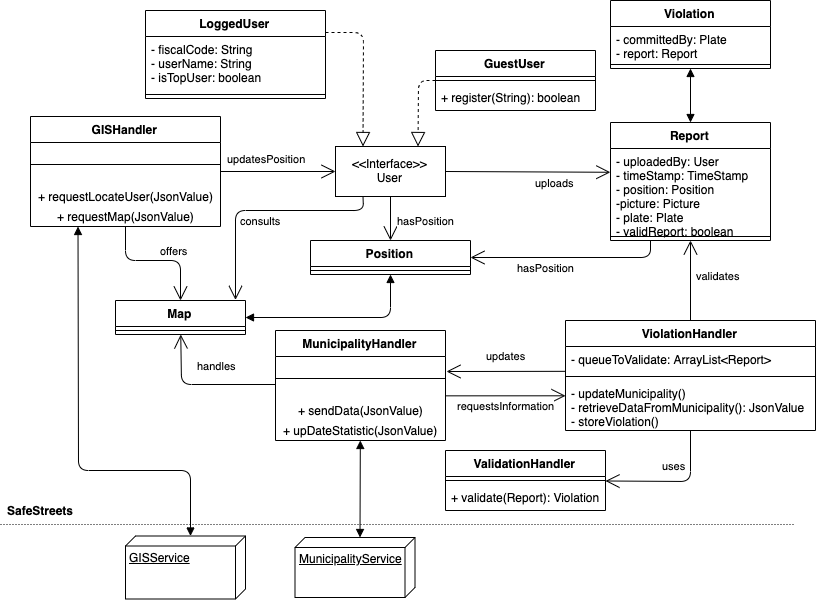
\includegraphics[width=350pt, height=200pt]{diagrams/uml.png}
			\caption{ 
				\label{fig:classDiagram} 
				SafeStreets Class Diagram
			}
		\end{figure}
		
	\subsubsection{System Interfaces}
	\label{sec:systemInterfaces}
		The system requires some external interfaces (represented in \autoref{fig:systemInterfaces}) to accomplish the \hyperref[sec:goals]{goals stated before}. \newline 
		\begin{figure}[h]
			\centering
			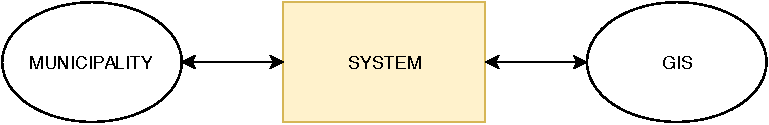
\includegraphics[width=300pt, height=50pt]{diagrams/system_blocks}
			\caption{
				\label{fig:systemInterfaces} 
				Overview of system interfaces
			}
		\end{figure} 
\clearpage			
\paragraph{Municipality Data Exchange} The system will interact with municipalities. The system will retrieve the information about the accidents that occur on the territory of the municipality and cross this information with its own data to identify potentially unsafe areas. It will also retrieve the information about issued tickets from the municipalities to build statistics, for example about the effectiveness of the SafeStreets initiative (e.g., by looking for trends in the issuing of tickets). In addition, our system will expose via a \emph{restricted access API} the stored information about the violations to the municipalities, so that the local authorities can generate traffic tickets from it, and receive suggestions for possible interventions (e.g., add a barrier between the bike lane and the part of the road for motorised vehicles to prevent unsafe parking). \cite{Assignments}


\label{gis}	
\paragraph{Geographic Information System} The system will interact with an external GIS. Our system will map the spatial location of stored violations and visualise the spatial relationships among them. The external GIS will map quantities, such as where the most and least number of violations occurred, to find places that meet the user requested criteria inside an area of interest. This can be accomplished mapping concentrations, or a quantity normalised by area or total number. The system can map the change in a specific geographic area to visualise statistics, or to evaluate the results of the SafeStreets initiative.	

\subsubsection{User Interfaces}
\label{sec:userinterfaces}

The system requires a user interface as the access point where users interact with the system. As the user interface design can dramatically affect the usability and user experience of the system, the layout of the user interface will be clearly set out so that elements can be found in a logical position, in a way that users will be able to find the the information and services they are looking for.

\paragraph{Guest User}
	Using the user interfaces of the system guest users can:
	\begin{itemize}
		\item Register to the system
		\item Authenticate and log-in to the system
	\end{itemize}
	
\paragraph{Logged User}
	Using the user interfaces of the system logged users can:
	\begin{itemize}
		\item Submit a violation with all the required and optional metadata
		\item Consult a map through an external GIS visualising specific data based on a selected criteria
		\item Consult different statistics generated upon the system and the municipality collected data
		\item View and edit personal information
	\end{itemize}
		
\subsubsection{Hardware Interfaces}
\label{sec:hardwareinterfaces}
	The system will interact with the user's device hardware interfaces.	
	\begin{itemize} 
		\item Telephony and other wireless connections are leveraged for the communication between the user and the system
		\item Full access to the user's device camera hardware is needed for the user to capture a photo
		\item The geomagnetic field sensor and the proximity hardware-based sensor are leveraged to determine the position of the user's device
	\end{itemize}

\subsubsection{Software Interfaces}
	In order to accomplish the \hyperref[sec:goals]{goals stated before} the system requires to interface with Databases and DBMSs, required in order to store data about users, violations, and the corresponding metadata. These interfaces are also required to guarantee the ability to input queries to the database in order to satisfy the system required capabilities.
	
\subsubsection{Communication Interfaces}
	The system requires secure communication within the involved entities in a way not susceptible to eavesdropping or interception. Secure communication includes means by which the system can share information that third parties cannot intercept or alter. For these reasons communication encryption methods must be implemented in a way that guarantees the use of encryption, i.e. if encrypted communication is impossible then no traffic is sent.

\subsection{Product Functions}
\paragraph{Violation Upload Procedure} 
Provide logged users with the ability to notify authorities when traffic violations occur and, in particular, parking violations. The application allows users to send pictures of violations, including the suitable required metadata. In particular, when it receives a picture, it runs an algorithm to read the license plate number (the user can help with the recognition via an optional form) and it stores the retrieved information with the violation, including also the type of the violation (submitted by the user) and the street where the violation occurred. \cite{Assignments}

\clearpage

	\begin{figure}[h]
		\centering
		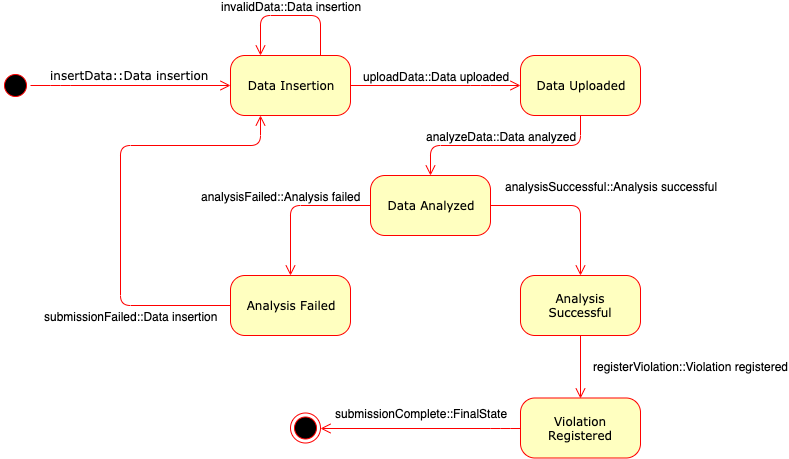
\includegraphics[width=320pt]{diagrams/state-diagrams/SubmitViolation.png}
		\caption{
			\label{fig:violationUpload} Violation Upload Process
		}
	\end{figure}
	
\paragraph{Retrieve Data from Municipality}
Retrieve the information about the accidents that occur on the territory and the issued tickets using the service offered by the municipalities and cross this data with SafeStreets data to identify potentially unsafe areas and build different types of statistics. This will also allow the system to understand which violations are more likely to cause accidents in a particular zone and elaborate suggestions on possible interventions, later communicated to the municipality via a \emph{restricted access API} provided to them. \cite{Assignments} \newline

	\begin{figure}[h]
		\centering
		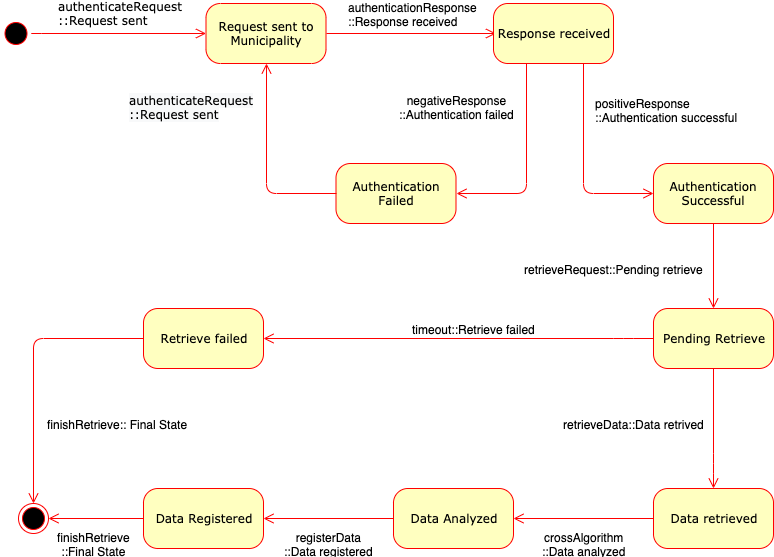
\includegraphics[width=285pt, height=205pt]{diagrams/state-diagrams/RequestMunicipality.png}
		\caption{
			\label{fig:retrieveMunicipality} Retrieve Data From Municipality}
	\end{figure}
	
\clearpage

\paragraph{Show Information and Statistics}
The application allows logged users to mine the information that has been received, highlighting the streets (or the areas) with the highest frequency of violations, considered unsafe areas, or the vehicles that commit the most violations. In addition, statistics about issued tickets, or the effectiveness of the SafeStreets initiative, are shown to the user if requested. \cite{Assignments} \newline
	\begin{figure}[h]
		\centering
		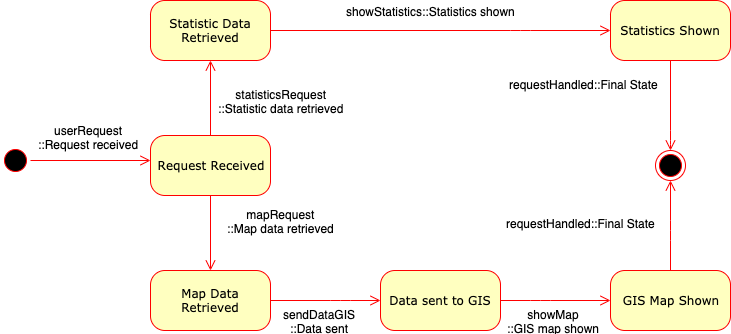
\includegraphics[width=300pt, height=135pt]{diagrams/state-diagrams/ShowStatistics.png}
		\caption{
			\label{fig:showStatistics} Show Information and Statistics
			}
	\end{figure}
	
\paragraph{Restricted Access API}
The system will expose via a \emph{restricted access API} the stored information about the violations to the municipalities, so that the local authorities can generate traffic tickets from it and receive suggestions for possible interventions to carry out (e.g., add a barrier between the bike lane and the part of the road for motorised vehicles to prevent unsafe parking), in order to decrease the risk of those areas, increasing their safety. \cite{Assignments} \newline
	\begin{figure}[h]
		\centering
		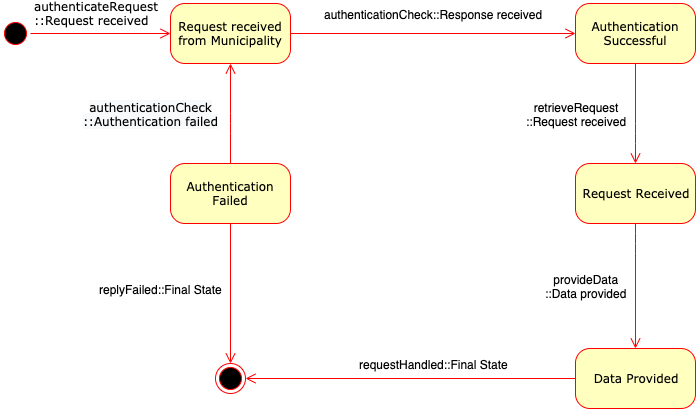
\includegraphics[width=300pt, height=170pt]{diagrams/state-diagrams/RequestAPI.png}
		\caption{
			\label{fig:restrictedAPI} Restricted access API
		}
	\end{figure}


\subsection{User Characteristics}
	Users can use our system when they notice a violation and want to communicate it to the authorities. Necessary conditions for the user in order to use the system are:
 	\begin{itemize}
 		\item The user must have a smartphone with a working connection to the internet and must be able to functionally use the provided services
 		\item The user must be in the age of majority in order to decrease the cases of wrong reports caused by user's inexperience on the topic 
 		\item A direct consequence of the previous item is that the user must be able to identify violations and the different types of violations
 	\end{itemize}
 	The user agrees to these conditions during the registration to the system.
 	
\subsection{Constraints}
\label{sec:constraints}
	We assume that these constraints are always met:
	\begin{enumerate}[label=\textbf{C\arabic*}]
		\item \label{constraint:accurateGPS} GPS position is supposed to be accurate (max error $\pm5$m)
		\item \label{constraint:pictureQuality} The quality of the picture is sufficient to recognise the plate number (min resolution 320x240)
		\item \label{constraint:strongConnection} Internet connection must be strong enough to allow the upload of the picture in a reasonable amount of time (supported technologies are 3G, 4G and 5G due to the performance requirement)
	\end{enumerate}
	
\subsection{Assumptions}
	We assume that these assumptions hold true in the domain of our system 
	\begin{enumerate}[label=\textbf{	DA\arabic*}]
		\item \label{assumption:obtainableGPS} GPS position of all users is always obtainable
		\item \label{assumption:workingConnection} Internet connection always works correctly
		\item \label{assumption:municipalityReachable} Municipality services are always reachable
		\item \label{assumption:mapsReachable} The maps provided by the GIS are always reachable and up to date
		\item \label{assumption:workingDBMS} The DBMS always works properly and the information in the DB are always accessible
		\item \label{assumption:smartphoneOS} The smartphone of the user runs iOS (9 or later) or Android (Jelly Bean or later)
		\end{enumerate}
		
\clearpage

\section{Specific Requirements}

\subsection{External Interfaces}

\subsubsection{System Interfaces}

\paragraph{Municipality Data Exchange} The definition of the municipality data exchange interface is dependent to the corresponding SafeStreet's interface required to be offered to the municipalities. The municipality is required to offer the following functionalities to the system:

	\begin{itemize}
		\item guarantee a secure authentication to the municipalities' system using a provided \emph{restricted access API}
		\item provide a secure transfer of data related to accidents occurred in the territory of the municipality
		\item provide a secure transfer of data related to local authorities' issued tickets 
	\end{itemize} 
	
	Leveraging the retrieved municipality data the system is required to cross this information with the system previously stored data. In addition, the system is required to perform the following functions on the crossed data:
	
	\begin{itemize}
		\item build statistics on the frequency of violations
		\item build statistics on the vehicles that commit the most violations
		\item build statistics on the most egregious offenders leveraging the issued tickets data
		\item build statistics on the effectiveness of the SafeStreets initiative by looking for trends in the issuing of tickets
		\item identify potentially unsafe areas and store this new generated information 
		\item identify possible interventions to be suggested to the municipalities and store this new generated information 
	\end{itemize}
		
	To fulfil the bidirectional data exchange the system is required to offer the following functionalities to the municipalities:
	
	\begin{itemize}
		\item guarantee a secure authentication to the system using a provided \emph{restricted access API}
		\item provide a secure transfer of data related to user uploaded violations and all the corresponding metadata
		\item provide a secure transfer of data related to possible interventions suggestions 
		
	\end{itemize} 
	
\clearpage

\paragraph{Geographic Information System} The definition of the external GIS interface is GIS dependant and will be described in a functionality-based way. The system is required to perform the following functions:

	\begin{itemize}
		\item load and filter data based on the user requested criteria
		\item cache retrieved data for the most common user requested criteria
		\item communicate the loaded and filtered data to the external GIS with the final goal of presenting the requested map to the user via the user interfaces
		
		\end{itemize}
	
	The system via the external GIS is required to be capable of handling the following data visualisations:
	
	\begin{itemize}
		\item visualise the spatial location of stored violations inside a specific geographic area requested by the user
		\item visualise the spatial location of stored violations inside a specific geographic area and a specific time range requested by the user
		\item visualise the distinction between possible safe and unsafe areas identified by the system
		\item map quantities and concentrations, such as where the most and least number of violations occurred, highlighting the streets (and areas) with the highest frequency of violations
		\item map the change of quantities and concentrations inside a specific geographic area and a specific time range requested by the user
	\end{itemize}

	\begin{figure}[h]
		\centering
		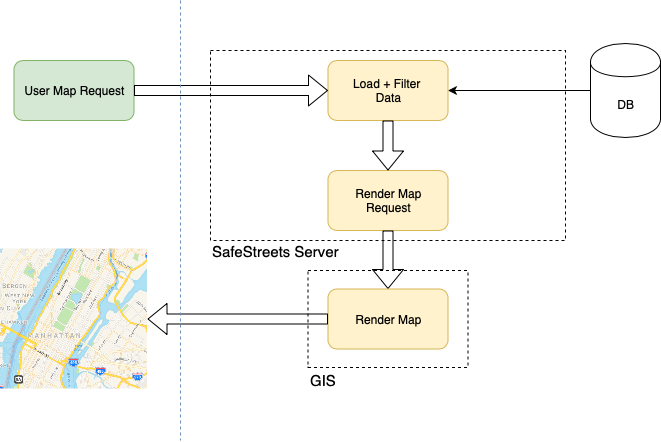
\includegraphics[width=320pt]{diagrams/GIS.png}
		\caption{
			\label{fig:externalGIS} GIS Interaction Diagram}
	\end{figure}

\subsubsection{User Interfaces}
\label{sec:userinterface}

\subsubsection{Hardware Interfaces}
\subsubsection{Software Interfaces}
\subsubsection{Communication Interfaces}


\subsection{Functional Requirements}
Definition of use case diagrams, use cases and associated sequence/activity diagrams, and mapping on requirements

\subsection{Performance Requirements}

\subsection{Logical Database Requirements}

\subsection{Design Constraints}

\subsubsection{Standards Compliance}
\subsubsection{Hardware Limitations}
\subsubsection{Other?}

\subsection{Software System Attributes}

\subsubsection{Reliability}
\subsubsection{Availability}
\subsubsection{Security}
\subsubsection{Maintainability}
\subsubsection{Portability}





\subsection{Functional Requirements}
The following requirements are derived in order to achieve the specified goals.
\subsubsection{Goals}
	\begin{description}
		\item \ref{goal:register}\ Allow guest users to register to the system
			\begin{enumerate}[label=\textbf{R\arabic*}]
			
  				\item The system must require the \emph{guest} user to insert his fiscal code, a username, a valid e-mail and a password to identify him
  				
   				\item The system must check that the validity of the data inserted by the \emph{guest} user namely avoid duplicates, invalid fiscal codes and too weak passwords
   				
   				\item The system must send an e-mail to the \emph{guest} user to verify the e-mail address given during the registration
   
  			\end{enumerate}
  				
				\textbf{DA2} Internet connection always works correctly
				
				\textbf{DA6} The smartphone of the user runs iOS (9 or later) or Android (Jelly Bean or later)
			
  			
		\item \ref{goal:login}\ Allow registered users to authenticate to the system
			\begin{enumerate}[label=\textbf{R\arabic*}, resume]
  				\item The system must require the user to insert his username and password to authenticate to the system
   				\item The system must be able to check if the username and password pair correspond to a user correctly registered to the system and grant the access to that user

			\end{enumerate}
			
			\textbf{DA2} Internet connection always works correctly
			
			\textbf{DA5} The DBMS always works properly so that the information in the DB are always accessible
			
		\item \ref{goal:userTransfer}\ Allow users to transfer data to the system describing occurred violations, including the suitable metadata to describe the submitted violation			\begin{enumerate}[resume*]
				\item The system must allow the user to take a picture of the violation and the plate from the mobile application
  				\item The system must allow the user to manually insert the license plate number in order to help the recognition algorithm
  				\item The system must be able to retrieve the license plate of the vehicle running an algorithm to recognise it
  				\item The system must be able to verify that the license plate number is valid and registered to a vehicle
  				\item The system must require the user to specify the type of violation
  				\item The system must allow the user to provide the location of the violation, manually specifying the address, picking it up from the map or using the GPS of the device
   			\end{enumerate}
   			
   			\textbf{C2} The quality of the picture is sufficient to recognise the plate number (min resolution 320x240)
   			
			\textbf{C3} Internet connection must be strong enough to allow the upload of the picture in a reasonable amount of time (supported technologies are 3G, 4G and 5G due to the performance requirement)
			
			\textbf{DA1} GPS position of all users is always obtainable
			
			\textbf{DA2} Internet connection always works correctly
			
		\item \ref{goal:avoidLeaks}\ Ensure that the chain of custody of the information provided by the users is never broken, and the information is never altered or manipulated			\begin{enumerate}[resume*]
   				\item The system must provide a secure channel to communicate with the users
   				\item The system must encrypt the connection with the users in order to protect the process of providing data
   				\item The system must adopt security measures to prevent malicious accesses and to protect sensible data
   				\item Questo davvero non lo so mori miei
  			\end{enumerate}
  			
  			
		
		\item \ref{goal:municipalityTransfer}\ Allow the system to retrieve data about the accidents that occur on the territory and data about issued tickets via the municipality provided service
			\begin{enumerate}[resume*]
   				\item The system must be able to retrieve data about accidents from municipality systems 
   				\item The system must be able to process data retrieved from municipality
   				\item The system must be able to elaborate accidents and violations information to extract data about unsafe areas
   				\item The system must be able to provide data to municipality systems to suggest possible interventions to increase safety in a specific area
  			\end{enumerate}
  			
  			\textbf{DA2} Internet connection always works correctly
  			
			\textbf{DA3} Municipality services are always reachable
  			
  		\item \ref{goal:statistics}\ Allow the system to cross the information submitted by the users and the information retrieved from the municipality to build statistics
  			\begin{enumerate}[resume*]
  				\item 
   				
  			\end{enumerate}
  		\item \ref{goal:consultMap}\ Allow users to consult a map highlighting the streets (and the areas) with the highest frequency of violations, the identified potentially unsafe areas and view statistics about previously stored violations
  			\begin{enumerate}[resume*] 
  				\item The system must be able to retrieve data about tickets issued by the municipality 
   				\item The system must be able to process data retrieved from municipality
   				\item The system must be able to elaborate issued tickets information to generate statistics about useful violations provided by users
   			\end{enumerate}
   			
   			\item \ref{goal:retrieveData}Allow municipality to consult the system data and receive suggestions on possible interventions via a restrict access API 
   				\begin{enumerate}[resume*] 
  				\item The system must be able to retrieve data about tickets issued by the municipality 
   				\item The system must be able to process data retrieved from municipality
   				\item The system must be able to elaborate issued tickets information to generate statistics about useful violations provided by users
   			\end{enumerate}
   			
   	\end{description}
  	
\subsection{Performance Requirements}
	The system should ensure acceptable response times in the interactions with the user, which strictly depends on the number of concurrent users and the connection speed.
\newline
The processes of providing data and loading the map of safe and unsafe areas shouldn't be too slow.
\subsection{Software System Attributes}
	\subsubsection{Availability}
	The system must be available 99,9\% of the time (up to 8,76 hours per year of downtime). The system should be accessible 24 hours per day.
	\subsubsection{Security}
	Users personal information and payment information are encrypted and must be protected during transmission, as already stated the PTPP protocol will be used to ensure encryption through the network.
	Restricted access APIs must check that who tries to use them is actually allowed to do so.
	\subsubsection{Portability}
	The system must be also accessible by the most common mobile platforms (iOS and Android devices).



\setlength{\parindent}{4ex}
\setlength{\parskip}{1ex}

\section{Formal Analysis using Alloy}

\subsection{Source code}
		\lstinputlisting[language=alloy]{alloy/SafeStreets.als}

\clearpage
\subsection{Generated Worlds}

\begin{figure}[h!]
	\centering
	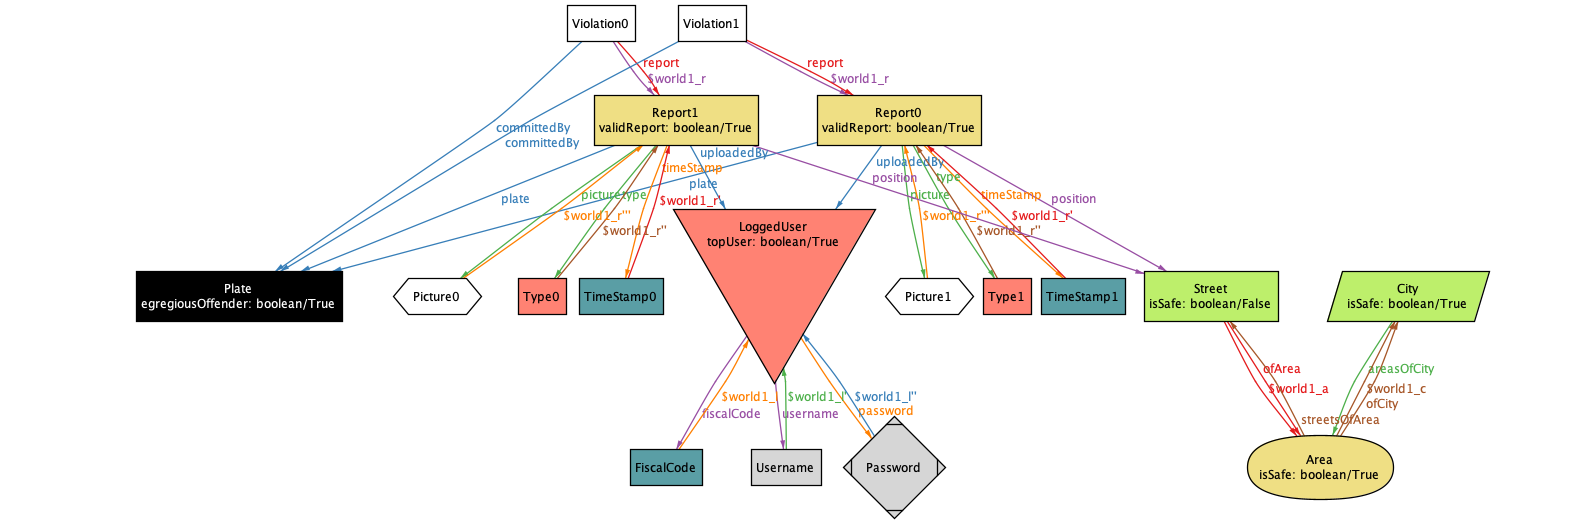
\includegraphics [height=170pt,angle=-90]{alloy/world1.png}
	\caption{
		\label{fig:World1} 
		World 1
	}
\end{figure}

\begin{figure}[h!]
	\centering
	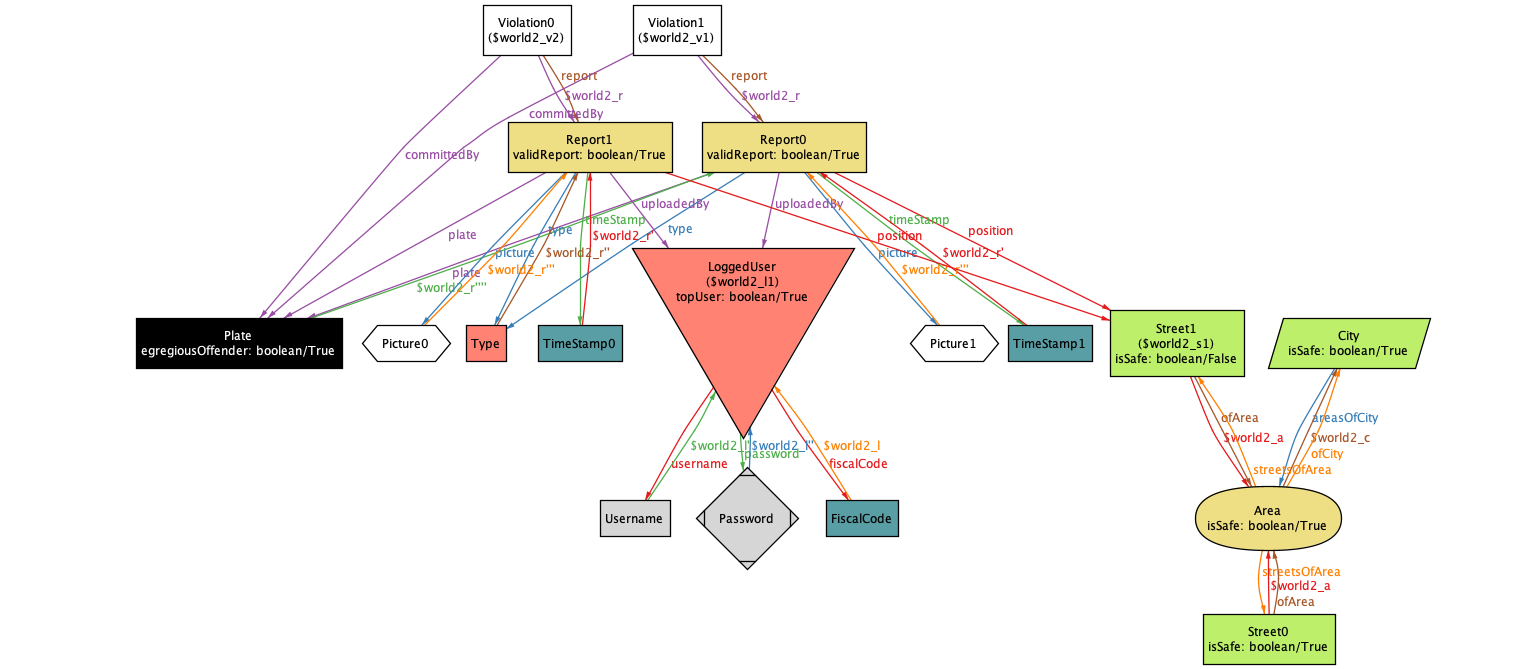
\includegraphics [height=230pt,angle=-90]{alloy/world2.png}
	\caption{
		\label{fig:World2} 
		World 2
	}
\end{figure}

\begin{figure}[h!]
	\centering
	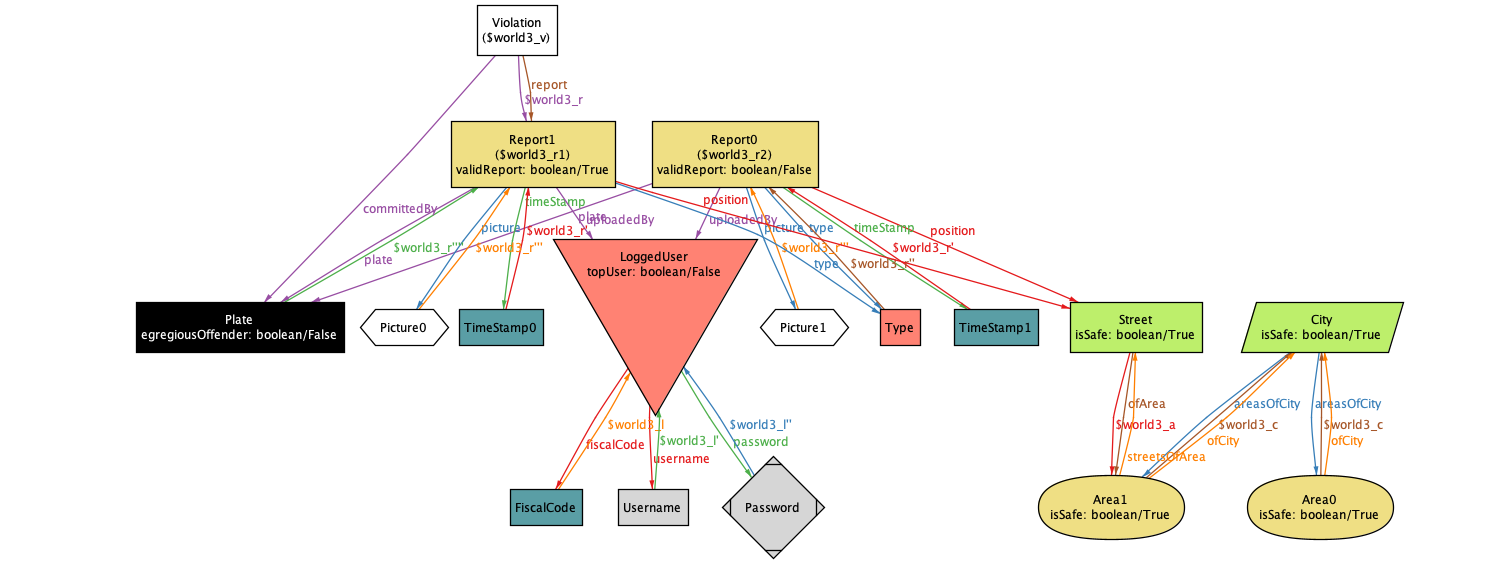
\includegraphics [height=200pt,angle=-90]{alloy/world3.png}
	\caption{
		\label{fig:World3} 
		World 3
	}
\end{figure}

\begin{figure}[h!]
	\centering
	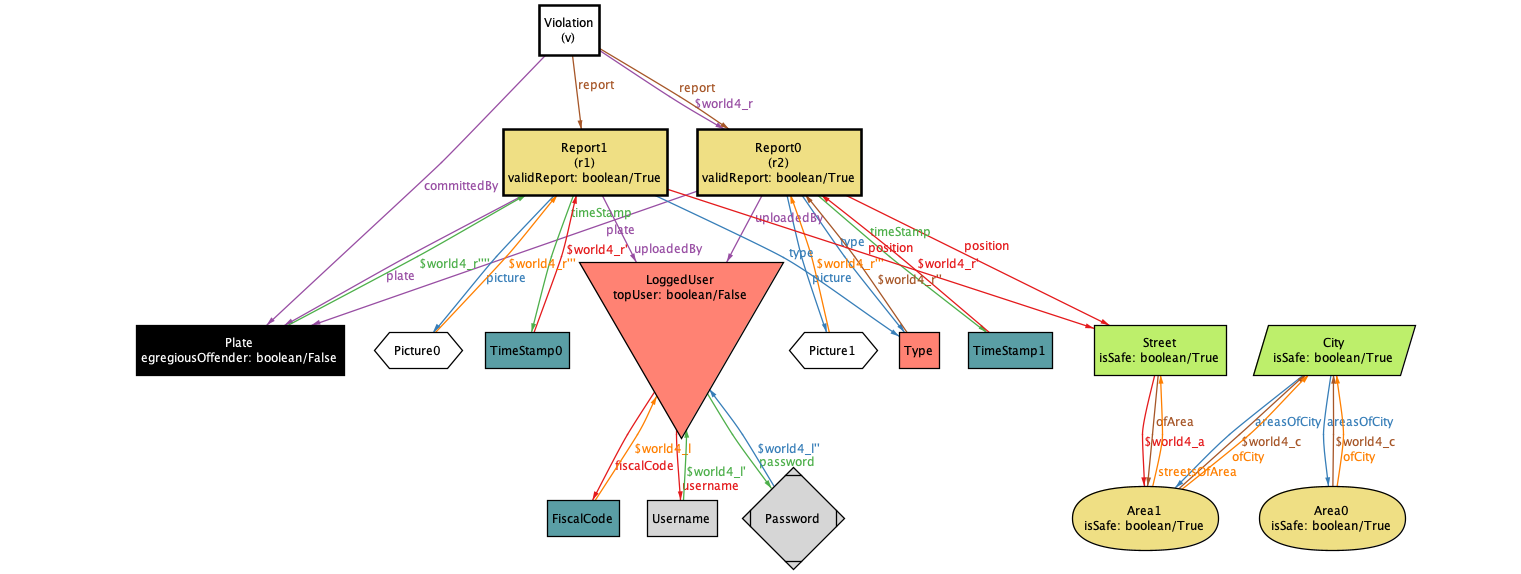
\includegraphics [height=200pt,angle=-90]{alloy/world4.png}
	\caption{
		\label{fig:World4} 
		World 4
	}
\end{figure}

\begin{figure}[h!]
	\centering
	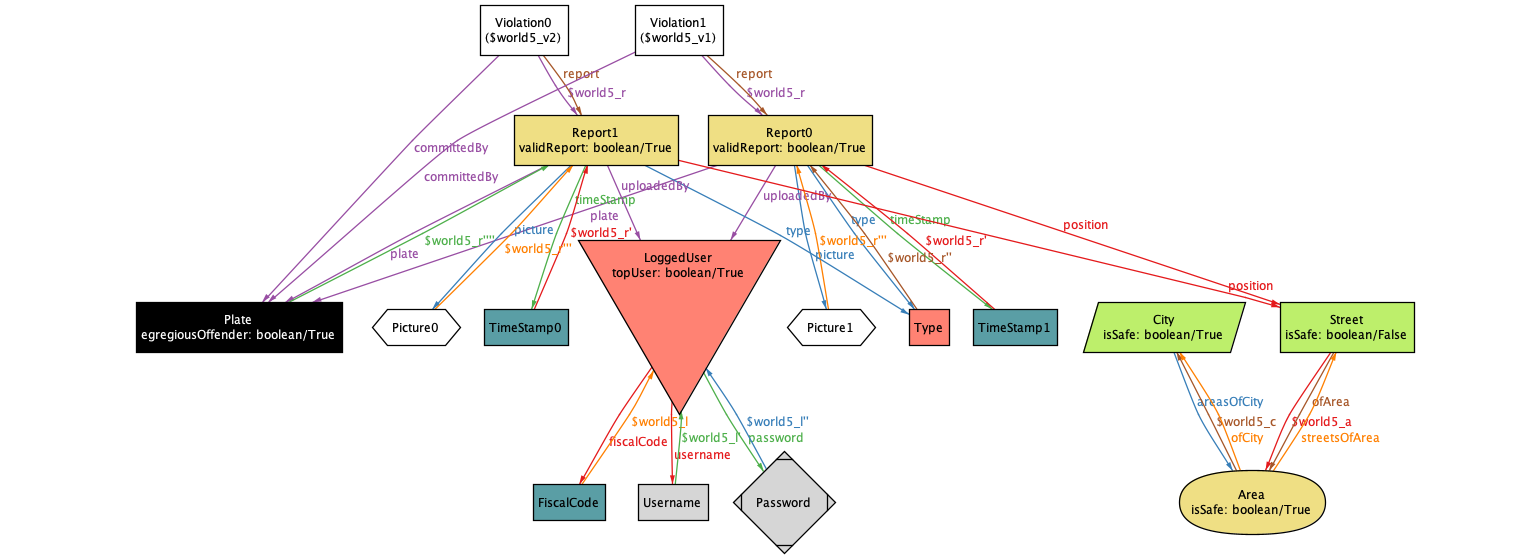
\includegraphics [height=200pt,angle=-90]{alloy/world5.png}
	\caption{
		\label{fig:World5} 
		World 5
	}
\end{figure}

\clearpage

\paragraph{Notes to read the generated worlds}
	\begin{itemize}
		\item The generated \hyperref[fig:World1]{World 1} represents a possible situation in which a LoggedUser acquired the \emph{Top User} label, thanks to its high number of valid submissions.
		
		\item The generated \hyperref[fig:World2]{World 2} represents a possible situation in which Street1 acquired the \emph{Unsafe} label, due to its high number of violations. Street0 is considered \emph{Safe} since no violations occurred in that street.
		
		\item The generated \hyperref[fig:World3]{World 3} represents a possible situation in which Report0 didn't acquire the \emph{Valid Report} label, so it wasn't converted to a Violation.
		
		\item The generated \hyperref[fig:World4]{World 4} represents a possible situation in which two different reports (Report0 and Report1) described the same violation, so they are both connected to the same Violation instance.
		
		\item The generated \hyperref[fig:World5]{World 5} represents a possible situation in which the Plate acquired the \emph{Egregious Offender} label, since it committed two different violations (Violation0 and Violation1).
	\end{itemize}

\begin{appendices}

	\section{Alloy model}
		\subsection{Source code}
		\lstinputlisting[language=alloy]{alloy/alloy2.0version.als}
		\begin{figure}[h!]
			\centering
			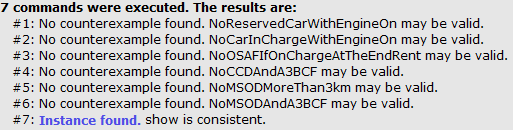
\includegraphics[]{alloy/AlloyResult.png}
			\caption{
				\label{fig:alloyExecutionResult} 
				Alloy execution result
			}
		\end{figure}
		\clearpage
		\subsection{Generated worlds}
			Note that in \autoref{fig:alloyWorld1} LoggedUser3 has been banned \emph{after} completing RentMade0.
			\begin{figure}[h!]
			\centering
			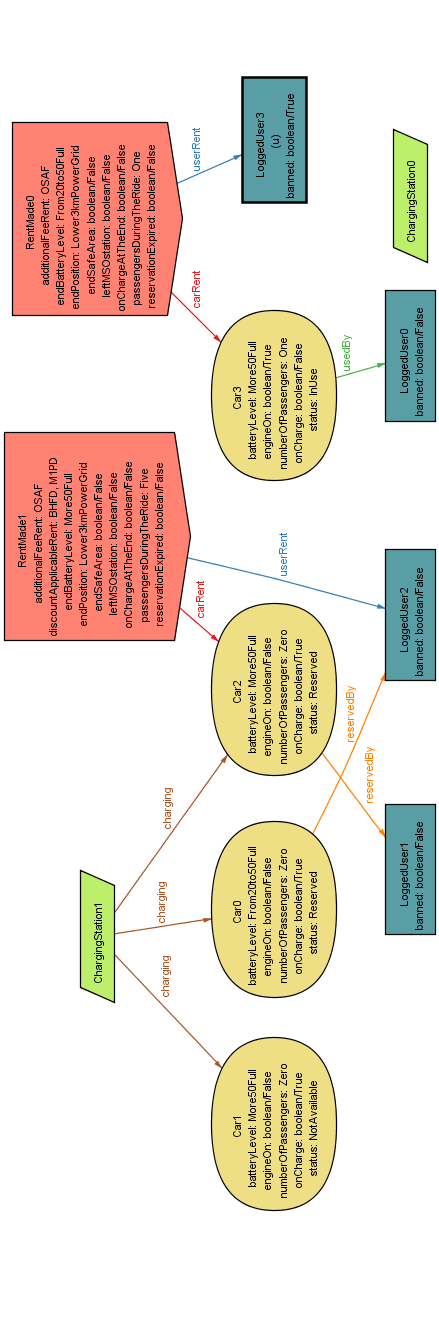
\includegraphics[scale=0.39]{alloy/AlloyWorld2.png}
			\caption{
				\label{fig:alloyWorld1} 
				First alloy generated world
			}
		\end{figure}
		\clearpage
		Note that in \autoref{fig:alloyWorld2} RentMade1 is actually a reservation expired of Car3 made by LoggedUser2. He now has reserved Car1.
		\begin{figure}[h!]
		\centering
		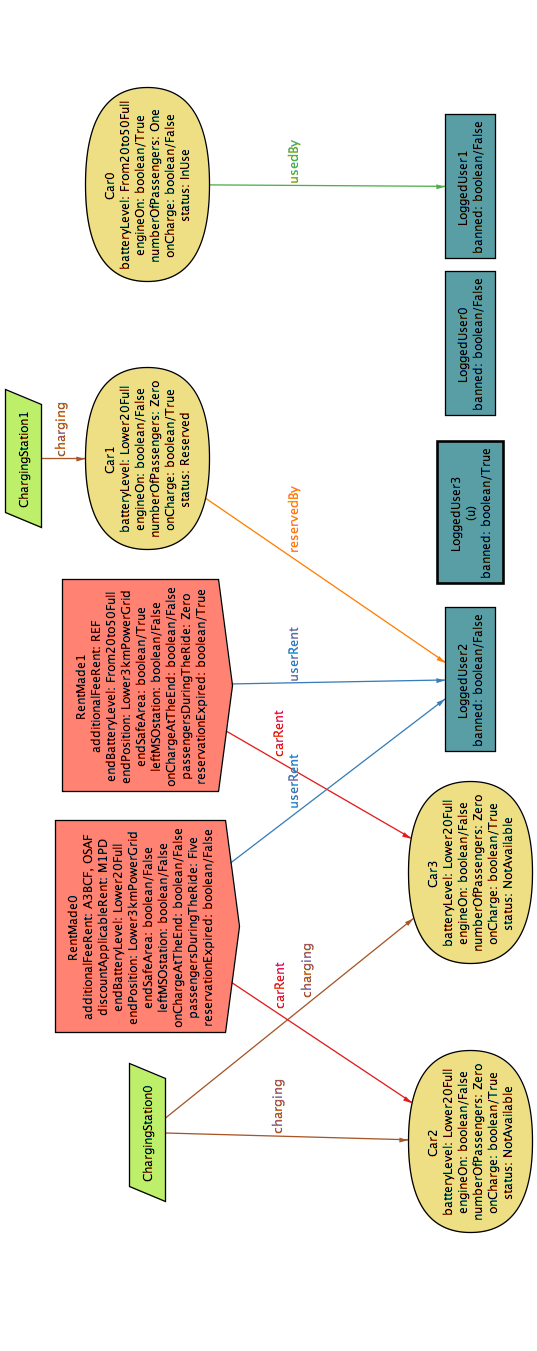
\includegraphics[scale=0.39]{alloy/AlloyWorld1.png}
		\caption{
			\label{fig:alloyWorld2} 
			Second alloy generated world
		}
		\end{figure}
		\clearpage
	\section{Software and tools used}
	For the development of this document we used
	\begin{itemize}
		\item \LaTeX{} as document preparation system
		\item \href{http://github.com}{GitHub} as version control system
		\item \href{http://draw.io}{Draw.io} for graphs
	\end{itemize}
		
	\section{Hours of Work}
	This is the amount of time spent to redact this document:
	\begin{itemize}
		\item \textbf{Section 1 - Introduction}
		\begin{itemize}
			\item Amedeo Cavallo - 2 hours
			\item Mattia Calabrese - 1 hour
			\item Federico Capaccio - 1 hour
		\end{itemize}
	\end{itemize}
	
	\section{Changelog}
	\begin{itemize}
		\item \textbf{v1.0} October 23, 2019
		\begin{itemize}
			\item Initial RASD document structuring and redaction
			\item Introduction (Purpose and Scope sections)
		\end{itemize}
	\end{itemize}
\end{appendices}
\clearpage
\begin{thebibliography}{9}
\bibitem{RE}B. Nuseibeh, S. Easterbrook, \emph{Requirements Engineering: A Roadmap}, 2000
\bibitem{Zave}P. Zave, \emph{Classification of Research Efforts in Requirements
Engineering}, ACM Computing Surveys, 1997
\bibitem{Assignments} E. Di Nitto, L. Mottola, \emph{Software Engineering 2 Assignment}, AA 2019-2020
\bibitem{Stone} A. Stone, “Chain of custody: How to ensure digital evidence stands up in court,” September 2015
\bibitem{IeeeRasd}IEEE Std 830:1993, \emph{IEEE Recommended Practice for Software Requirements Specifications}, 1993
\end{thebibliography}

\end{document}
